\chapter{Pengujian Terhadap Kode Program SIAModels}
\label{lamp:D}

\edef\vsiamodelsAIF {
	101,102,103,104,105,106,
	181,182,183,
	191,192,
	201,202,203,204,205,206,208,
	210,
	280,281,282,
	292,294,
	301,302,303,304,305,306,
	311,312,313,314,315,316,317,318,
	330,332,334,335,336,337,339,
	341,342,343,344,347,
	352,358,
	360,362,
	380,381,382,383,385,386,387,388,389,
	401,402,403,405,
	438,
	441,442,443,445,446,
	450,451,453,455,456,457,458,459,
	460,461,462,463,465,468,469,
	480,483,484,486}
\edef\vsiamodelsAKS{122,124}
\edef\vsiamodelsAMS{100,190,191,200,290}
\edef\vsiamodelsAPS{182,302,309,402}
\edef\vsiamodelsEAA{101,102}
\edef\vsiamodelsESA{101}
\edef\vsiamodelsESM{101,105,201,203,204}
\edef\vsiamodelsIIE{103,207,210,214}
\edef\vsiamodelsMKU{001,002,003,004,008,009,010,011,012}
\edef\vsiamodelsSIR{104}

\section{Kode Program}
\label{kodeProgram:D}
\lstinputlisting[language=Java, caption=Dosen.java]{./Lampiran/siamodels/Dosen.java}
\lstinputlisting[language=Java, caption=InfoMataKuliah.java]{./Lampiran/siamodels/InfoMataKuliah.java}
\lstinputlisting[language=Java, caption=JadwalKuliah.java]{./Lampiran/siamodels/JadwalKuliah.java}
\lstinputlisting[language=Java, caption=Mahasiswa.java]{./Lampiran/siamodels/Mahasiswa.java}
\lstinputlisting[language=Java, caption=MataKuliah.java]{./Lampiran/siamodels/MataKuliah.java}
\lstinputlisting[language=Java, caption=MataKuliahFactory.java]{./Lampiran/siamodels/MataKuliahFactory.java}
\lstinputlisting[language=Java, caption=Semester.java]{./Lampiran/siamodels/Semester.java}
\lstinputlisting[language=Java, caption=TahunSemester.java]{./Lampiran/siamodels/TahunSemester.java}

\lstinputlisting[language=Java, caption=HasPraktikum.java]{./Lampiran/siamodels/matakuliah/interfaces/HasPraktikum.java}
\lstinputlisting[language=Java, caption=HasPrasyarat.java]{./Lampiran/siamodels/matakuliah/interfaces/HasPrasyarat.java}
\lstinputlisting[language=Java, caption=HasResponsi.java]{./Lampiran/siamodels/matakuliah/interfaces/HasResponsi.java}

\lstinputlisting[language=Java, caption=Kelulusan.java]{./Lampiran/siamodels/prodi/teknikinformatika/Kelulusan.java}

\foreach \i in \vsiamodelsAIF {\lstinputlisting[language=Java, caption=AIF\i.java]{./Lampiran/siamodels/matakuliah/AIF\i.java}}
\foreach \i in \vsiamodelsAKS {\lstinputlisting[language=Java, caption=AKS\i.java]{./Lampiran/siamodels/matakuliah/AKS\i.java}}
\foreach \i in \vsiamodelsAMS {\lstinputlisting[language=Java, caption=AMS\i.java]{./Lampiran/siamodels/matakuliah/AMS\i.java}}
\foreach \i in\vsiamodelsAPS {\lstinputlisting[language=Java, caption=APS\i.java]{./Lampiran/siamodels/matakuliah/APS\i.java}}
\foreach \i in \vsiamodelsEAA {\lstinputlisting[language=Java, caption=EAA\i.java]{./Lampiran/siamodels/matakuliah/EAA\i.java}}
\foreach \i in \vsiamodelsESA {\lstinputlisting[language=Java, caption=ESA\i.java]{./Lampiran/siamodels/matakuliah/ESA\i.java}}
\foreach \i in \vsiamodelsESM {\lstinputlisting[language=Java, caption=ESM\i.java]{./Lampiran/siamodels/matakuliah/ESM\i.java}}
\foreach \i in \vsiamodelsIIE {\lstinputlisting[language=Java, caption=IIE\i.java]{./Lampiran/siamodels/matakuliah/IIE\i.java}}
\foreach \i in \vsiamodelsMKU {\lstinputlisting[language=Java, caption=MKU\i.java]{./Lampiran/siamodels/matakuliah/MKU\i.java}}
\foreach \i in \vsiamodelsSIR {\lstinputlisting[language=Java, caption=SIR\i.java]{./Lampiran/siamodels/matakuliah/SIR\i.java}}

\section{Hasil Latex}
\label{hasilLatex:D}
\lstinputlisting[language=TeX, caption=siamodels.tex]{./Lampiran/siamodels.tex}

\section{Hasil PDF}
\label{hasilPDF:D}
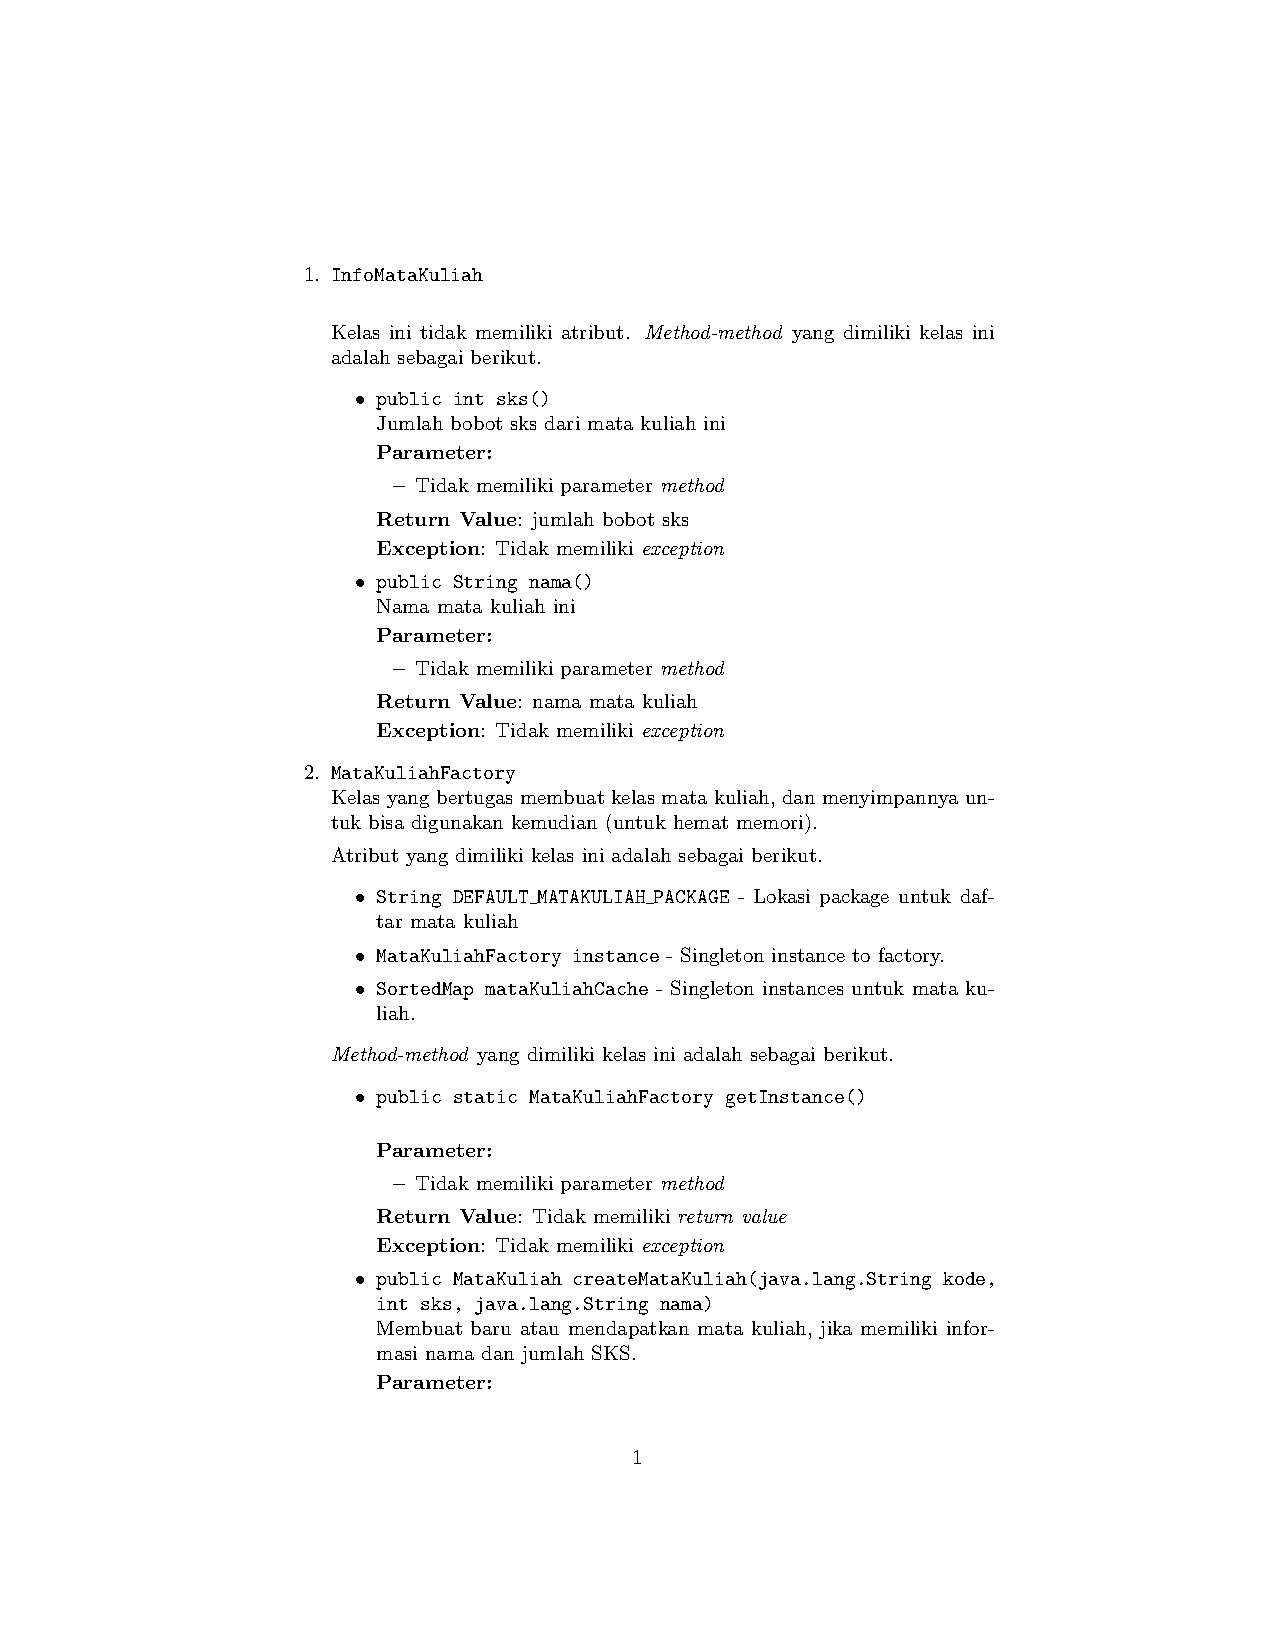
\includepdf[page=1-40]{./Lampiran/siamodels.pdf}
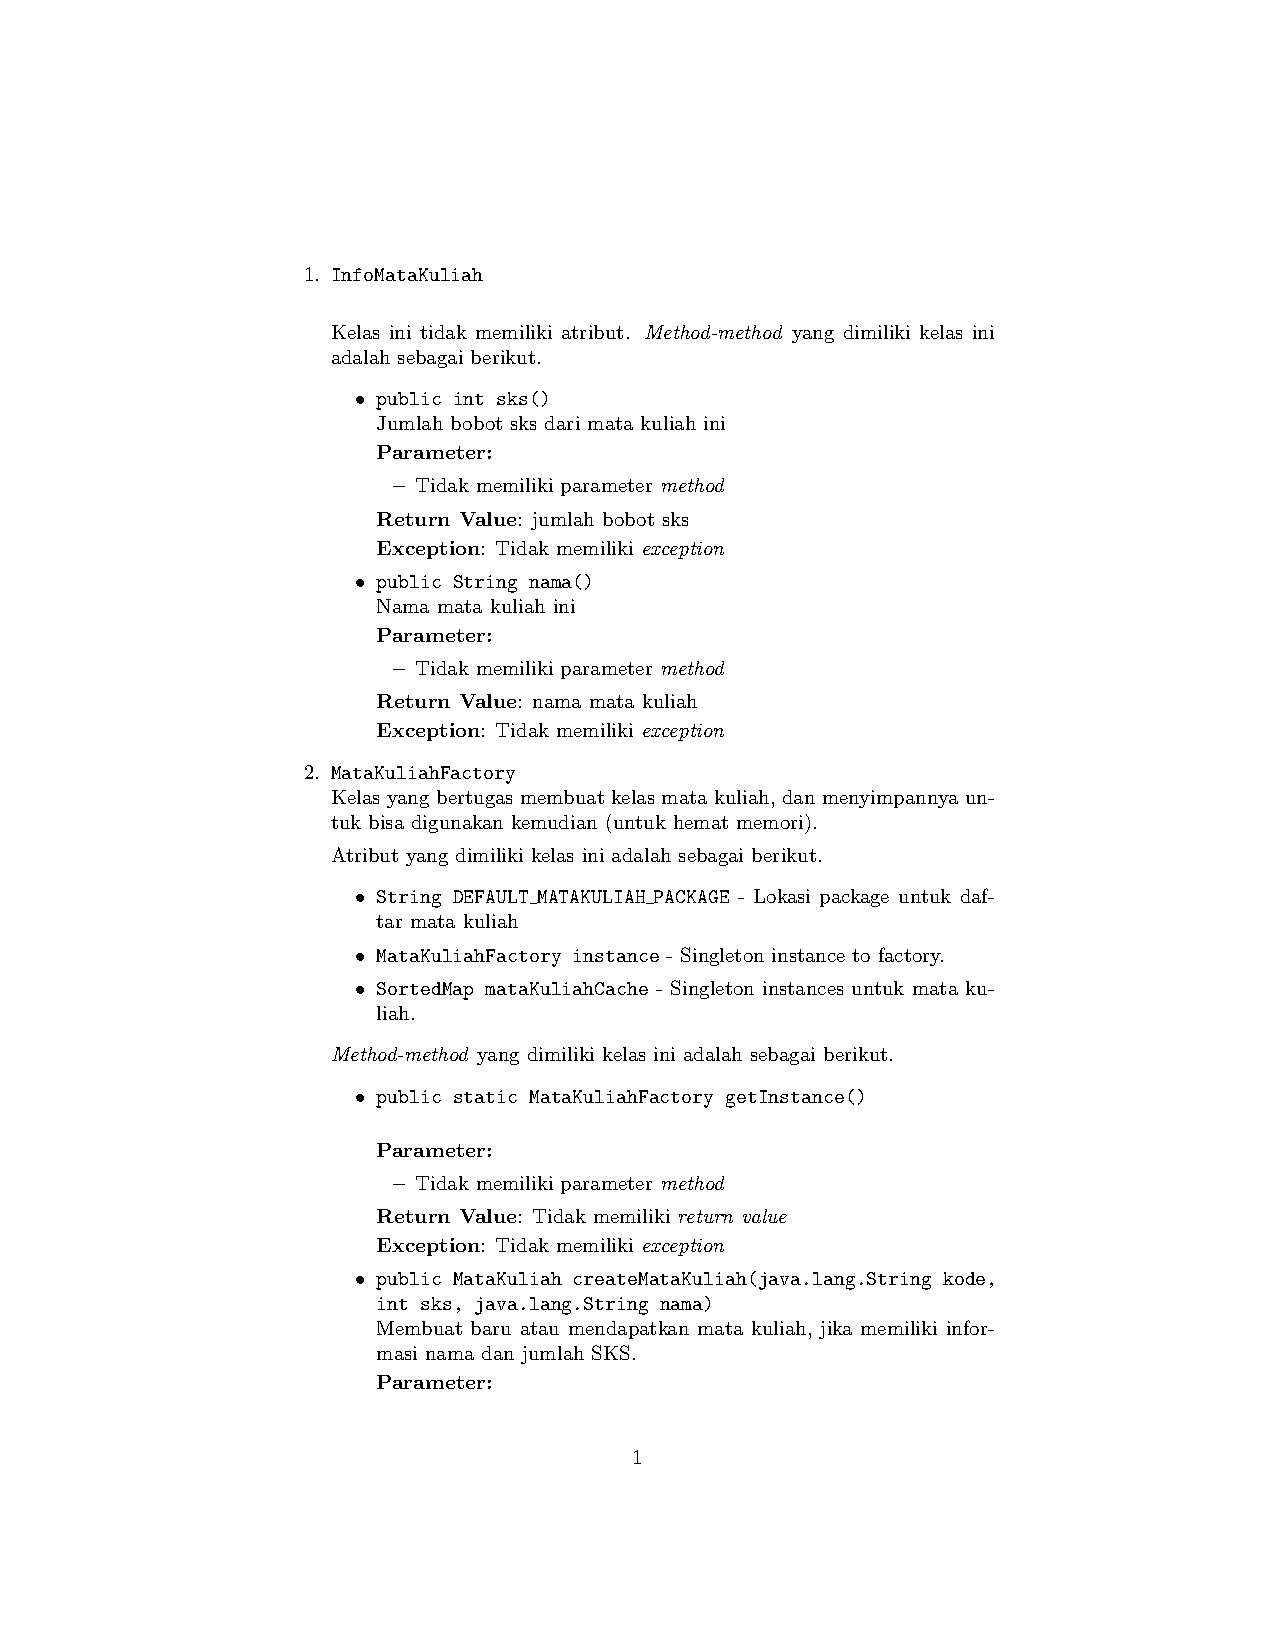
\includepdf[page=41,pagecommand={\null\vfill\captionof{figure}{javadoctolatex.pdf}}]{./Lampiran/siamodels.pdf}